\documentclass[aspectratio=169]{beamer}

\usetheme{Madrid}
\usecolortheme{default}
\setbeamertemplate{navigation symbols}{}
\setbeamertemplate{footline}[frame number]

\usepackage[utf8]{inputenc}
\usepackage[T1]{fontenc}
\usepackage{booktabs}
\usepackage{graphicx}
\usepackage{amsmath}
\usepackage{hyperref}
\usepackage{qrcode}

\title[Hopfield Energy for Hallucination Detection]{Do Attention-Derived Hopfield Energies Contain Hallucination Signal?}
\author{Evgenii Ivankin \\ MIPT}
\date{Study project}

\newcommand{\repoUrl}{https://github.com/eivankin/hopfield-energy-hallucination-detection}

\begin{document}

\begin{frame}
  \titlepage
\end{frame}

\begin{frame}{Problem}
  \begin{itemize}
    \item Hallucination detectors usually inspect generated text, external evidence, or model confidence.
    \item I ask a diagnostic question: can hallucination signal be seen inside the model's attention geometry?
    \item Focus: frozen language models, no finetuning of the base model.
  \end{itemize}

  \vspace{0.4cm}
  \begin{block}{Main claim}
    Q/K energy and attention-derived summaries contain transferable factuality signal, but scalar energy is not a universal hallucination score.
  \end{block}
\end{frame}

\begin{frame}{Hypothesis}
  \begin{columns}
    \begin{column}{0.56\linewidth}
      \begin{itemize}
        \item Transformer attention compares queries and keys.
        \item Modern Hopfield networks also perform associative retrieval through softmax similarity.
        \item If a response is weakly supported, its retrieval geometry may look different.
      \end{itemize}
    \end{column}
    \begin{column}{0.40\linewidth}
      \begin{equation*}
      E_t = -\sqrt{d_h}\log \sum_{i \le t}
      \exp\left(\frac{q_t^\top k_i}{\sqrt{d_h}}\right)
      \end{equation*}
      \centering
      \small Hopfield-style energy from attention Q/K states
    \end{column}
  \end{columns}
\end{frame}

\begin{frame}{Method}
  \begin{enumerate}
    \item Run frozen LLM on \texttt{prompt + response}.
    \item Extract Q/K tensors after RoPE from selected attention layers.
    \item Score response tokens only.
    \item Compute Hopfield energy summaries and prompt-attention summaries.
    \item Train simple logistic-regression probes with 5-fold CV.
  \end{enumerate}

  \vspace{0.25cm}
  \begin{block}{Baselines}
    Response length, response negative log-likelihood, and NLL + length.
  \end{block}
\end{frame}

\begin{frame}{Datasets and Models}
  \begin{table}
    \centering
    \small
    \begin{tabular}{lll}
      \toprule
      Dataset & Hallucination type & Models \\
      \midrule
      SMILES/SQuAD & context-grounded QA & Qwen2.5-0.5B \\
      RAGTruth & context-grounded RAG & Qwen2.5-0.5B, SmolLM2-360M, Gemma-3-1B \\
      TruthfulQA & open-domain false answers & Qwen2.5-0.5B \\
      \bottomrule
    \end{tabular}
  \end{table}

  \vspace{0.25cm}
  \begin{itemize}
    \item Learned probes are repeated over CV seeds: 13, 21, 42, 87, 101.
    \item AUROC is the main metric because hard-label F1 depends strongly on threshold calibration.
  \end{itemize}
\end{frame}

\begin{frame}{Main Result: Feature Families}
  \centering
  \IfFileExists{../final_report/figures/feature_family_auroc.pdf}{%
    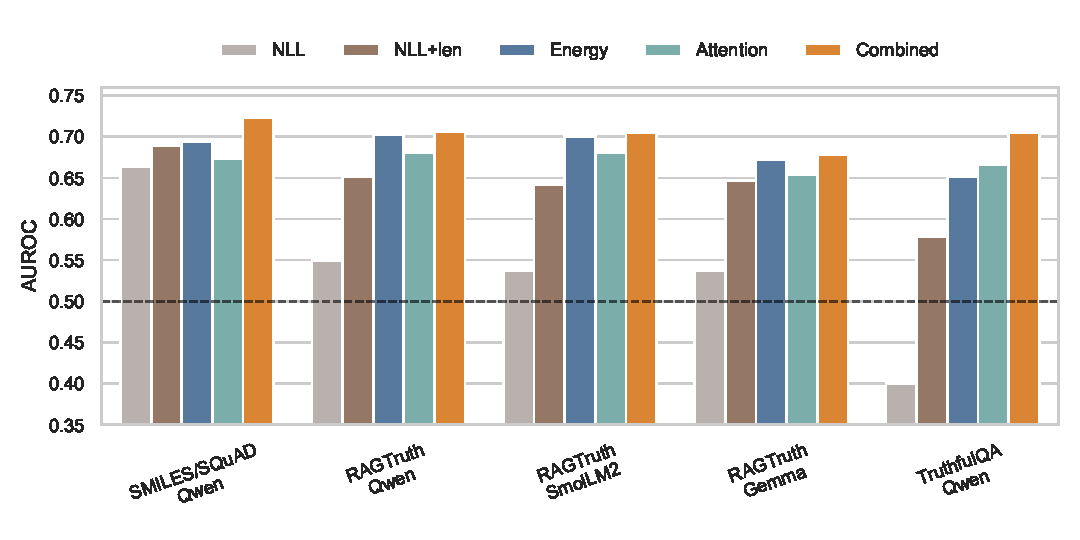
\includegraphics[width=0.90\linewidth]{../final_report/figures/feature_family_auroc.pdf}
  }{%
    \fbox{\parbox{0.82\linewidth}{Generate figures with \texttt{scripts/make\_final\_report\_figures.py}.}}
  }

  \small Combined Q/K-derived probes improve over response likelihood baselines.
\end{frame}

\begin{frame}{Transfer Across Models}
  \centering
  \IfFileExists{../final_report/figures/best_auroc_by_run.pdf}{%
    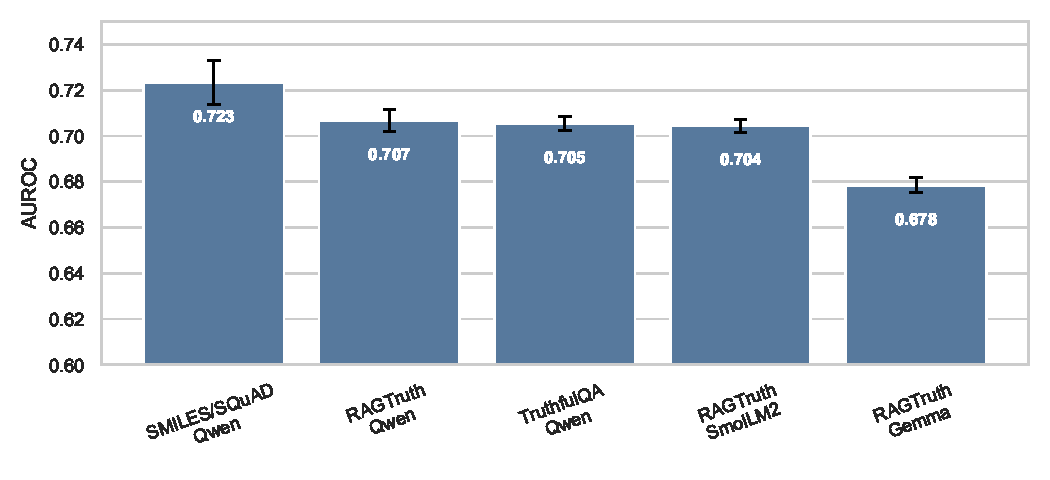
\includegraphics[width=0.90\linewidth]{../final_report/figures/best_auroc_by_run.pdf}
  }{%
    \fbox{\parbox{0.82\linewidth}{Generate figures with \texttt{scripts/make\_final\_report\_figures.py}.}}
  }

  \vspace{0.15cm}
  \small Qwen and SmolLM2 transfer strongly on RAGTruth; Gemma is weaker but remains above NLL/length.
\end{frame}

\begin{frame}{Important Caveat: Scalar Energy Direction}
  \centering
  \IfFileExists{../final_report/figures/scalar_energy_direction.pdf}{%
    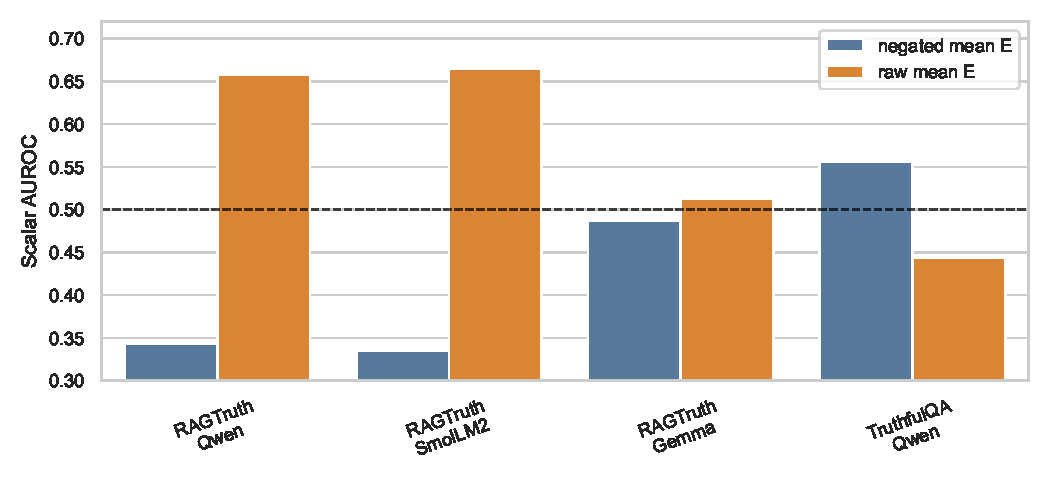
\includegraphics[width=0.90\linewidth]{../final_report/figures/scalar_energy_direction.pdf}
  }{%
    \fbox{\parbox{0.82\linewidth}{Generate figures with \texttt{scripts/make\_final\_report\_figures.py}.}}
  }

  \vspace{0.15cm}
  \small Scalar energy is not a universal monotonic hallucination score.
\end{frame}

\begin{frame}{Key Numbers}
  \begin{table}
    \centering
    \small
    \begin{tabular}{lr}
      \toprule
      Setting & Best AUROC mean $\pm$ std \\
      \midrule
      SMILES/SQuAD + Qwen2.5-0.5B & $0.723 \pm 0.010$ \\
      RAGTruth + Qwen2.5-0.5B & $0.707 \pm 0.005$ \\
      RAGTruth + SmolLM2-360M & $0.705 \pm 0.003$ \\
      RAGTruth + Gemma-3-1B & $0.679 \pm 0.003$ \\
      TruthfulQA + Qwen2.5-0.5B & $0.706 \pm 0.003$ \\
      \bottomrule
    \end{tabular}
  \end{table}

  \vspace{0.3cm}
  \begin{itemize}
    \item Stable across CV seeds.
    \item Strongest evidence: RAGTruth transfer from Qwen to SmolLM2.
    \item Weakest transfer: Gemma, suggesting architecture/layer sensitivity.
  \end{itemize}
\end{frame}

\begin{frame}{Conclusion}
  \begin{block}{What worked}
    Attention-derived Q/K energy and prompt-attention summaries contain hallucination/factuality signal beyond response likelihood.
  \end{block}

  \begin{block}{What did not become a universal rule}
    A single scalar rule like ``higher energy means hallucination'' is too strong.
  \end{block}

  \begin{block}{Next steps}
    Per-head analysis, layer sensitivity, larger models, and cleaner out-of-domain transfer tests.
  \end{block}
\end{frame}

\begin{frame}{Repository}
  \begin{columns}
    \begin{column}{0.55\linewidth}
      \Large Code, report, and reproduction commands

      \vspace{0.35cm}
      \normalsize
      \url{\repoUrl}

      \vspace{0.35cm}
      \begin{itemize}
        \item feature extraction
        \item public dataset conversion
        \item cached multi-seed evaluation
        \item final report and figures
      \end{itemize}
    \end{column}
    \begin{column}{0.38\linewidth}
      \centering
      \qrcode[height=5.1cm]{\repoUrl}
    \end{column}
  \end{columns}
\end{frame}

\end{document}
